Neutrinos were introduced into the \emph{Standard Model} as massless particles. But strong evidence from neutrino oscillation experiments indicates that at least one of the neutrino flavors has mass. Neutrino mass terms can be introduced into the \emph{Standard Model} within the Dirac or Majorana formalism. If the latter describes nature neutrinos are their own antiparticles. The constrain of neutrino mass scale comes from different aspects of physics. Cosmology gives constrain on the sum of masses of all the flavors. Single beta decay experiments measure the mass of the electron neutrino and sensitive to the neutrino mixing parameters. Neutrinoless double beta decay can only occur if neutrinos are of Majorana type. The decay rate would allow the determination of the effective Majorana neutrino mass. It gives information not only about neutrino mass scale, mixing parameters but also its intrinsic properties.

\section{Neutrinos in \emph{Standard Model}}
\label{sec:sm}
In the \emph{Standard Model} neutrinos are assumed to be fermions with spin 1/2 and rest mass $m_\nu=0$. They always have fixed helicity because there is no frame of reference moving faster than a neutrino, in which the helicity of the neutrino could change its sign. Neutrinos and anti-neutrinos are assumed to be different particles. Lepton numbers +1 and -1 are assigned to them respectively and the sum of which is conserved. Only left-handed neutrinos and right-handed anti-neutrinos participate in the weak interaction. The field operators of right-handed neutrinos and left-handed anti-neutrinos do not exist in the Lagrangian density of weak interaction at all.

New experimental evidence, particularly neutrino oscillations, make a modification and extension of the \emph{Standard Model} necessary. Crucial theoretical considerations and experimental observations are briefly reviewed in the following.

The neutrino was postulated to exist by W. Pauli in 1930~\cite{Pau30} in order to explain the continuous energy spectrum of electrons emitted from beta decay without abandoning the law of energy conservation. He assumed that it was a neutral fermion with spin 1/2, and its mass was of the same order of magnitude as the electron mass. E.  Fermi soon developed his theory of beta decay according to the beta spectrum~\cite{Fer33,Fer34}. He investigated the influence of the neutrino mass on the shape of beta spectrum and inferred that $m_\nu \approx 0$ by comparing the calculation with the experimental data. A precise measurement of the beta spectrum of tritium by L. Langer and R. Moffat in 1952~\cite{Lan52} gave an upper limit on the rest mass of the neutrino, $m_\nu < 250 \mbox{eV} = 0.002m_e$. The neutrino was assumed to be massless afterwards. Although the upper limit was pushed down again and again by later experiments, the possibility that neutrinos have very small masses was never completely ruled out, and was strongly supported by the neutrino oscillation experiments.

Beta plus decay was observed in artificial radioactivity by I. Curie and J. F. Joliot in early 1934~\cite{Cur34}. Beta decay and beta plus decay in a nucleus can be noted as follows:
\begin{equation}
  \label{eq:bd}
  \beta\mbox{-decay: } n \rightarrow p+e^{-}+\bar{\nu}_e ,
\end{equation}
\begin{equation}
  \label{eq:bpd}
  \beta^+\mbox{-decay: } p \rightarrow n+e^{+}+\nu_e .
\end{equation}
According to Fermi's theory, the following processes should also exist:
\begin{equation}
  \label{eq:enab}
  e^{+} + n \rightarrow p + \bar{\nu}_e ,
\end{equation}
\begin{equation}
  \label{eq:epab}
  e^{-} + p \rightarrow n + \nu_e ,
\end{equation}
where instead of $e^{-/+}$ emission, the absorption of $e^{+/-}$ occurs now. Process~\ref{eq:epab} occurring in a nucleus is called electron capture (EC in short), which was observed by L. W. Alvarez in 1938~\cite{Alv38}. The inverse process of \ref{eq:enab} was used by F. Reines and C. L. Cowan, Jr. to detect the neutrinos from nuclear reactors~\cite{Cow56, Rei56}. They proved at the first time that the neutrino does exist in nature.

Whether the neutrino accompanying with $e^{+}$ and the one accompanying with $e^{-}$ are the same particles was of great interest at that time. Consider the inverse process of EC,
\begin{equation}
  \label{eq:nunab}
  \nu_e + n \rightarrow p + e^{-} ,
\end{equation}
which, theoretically speaking, should also exist~\footnote{The process was proved to be exist experimentally and used to detect solar neutrinos in many experiments.}. If $\bar{\nu}$ and $\nu$ are the same, the following reaction, where $\nu_e$ is replaced by $\bar{\nu}$, could happen:
\begin{equation}
  \label{eq:bnun}
  \bar{\nu}_e + n \rightarrow p + e^{-}.
\end{equation}
This was investigated by R. Davis in 1955~\cite{Dav55,Dav56}. He was looking for
\begin{equation}
  \label{eq:bnucl}
  \bar{\nu}_e + ^{37}\mbox{Cl} \rightarrow ^{37}\mbox{Ar}+e^{-}
\end{equation}
and gave a negative result. Before the observation of parity violation and neutrino oscillations this result supported the idea that $\bar{\nu}$ and $\nu$ are intrinsically different particles. To formulate this idea theoretically different \emph{lepton numbers} were assigned to $e^{-}, e^{+}, \nu_e$ and $\bar{\nu}_e$:
\begin{equation}
  \label{eq:ln}
  +1 \mbox{ for }e^{-}, \nu_e, \mbox{   }-1 \mbox{ for
}e^{+},\bar{\nu}_e,
\end{equation}
and required to be conserved in the interaction. The reaction described by eq. \ref{eq:bnucl} is forbidden otherwise the \emph{lepton number} would change.

In 1956 T. D. Lee and C. N. Yang found the existing evidence of parity conservation in weak interaction unsatisfactory and specified the experiments required to check it~\cite{Lee56}. Soon after parity violation was observed in the beta decay of $^{60}$Co~\cite{Wu57} and the creation and decay of muons~\cite{Gar57,Fri57}. Lee and Yang~\cite{Lee57} and some other authors~\cite{Sal57,Lan57} started to apply the so-called two-component model~\cite{Wey29} to the weak interaction. According to this model only the left-handed neutrino and right-handed anti-neutrino or right-handed neutrino and left-handed anti-neutrino participate the weak interaction. In 1958 an elegant experiment was carried out by M. Goldhaber \textit{et al.} to see whether the right-handed or left-handed components were preferred by nature~\cite{Gol58}. By measuring the polarization of $\gamma$-rays emitted from $^{152}$Sm* created in the electron capture, $^{152}$Eu$(e^-,\nu)$, they inferred that neutrinos from $^{152}$Eu$(e^-,\nu)$ were left-handed. Now the absence of reaction \ref{eq:bnucl} could be explained in two different ways:
\begin{itemize}
\item $\bar{\nu}$ and $\nu$ behave different because they are   intrinsically different particles.
\item $\bar{\nu}$ and $\nu$ behave different only because they have   different helicities.
\end{itemize}

In summary, though the \emph{Standard Model} of weak interaction is a very successful theory some modifications are still possible:
\begin{itemize}
\item neutrinos could be massive;
\item $\bar{\nu}$ and $\nu$ might not be totally different, and hence   the \emph{lepton number} is not conserved.
\end{itemize}


\section{Neutrino oscillations}
\label{sec:osci}
The assumption that neutrinos were massless was challenged in 1969 by Gribov and Pontecorvo who predicted that neutrinos might oscillated into different flavors if some of them were massive and if there was mixing between them~\cite{Gri69}. This is what is called \emph{neutrino oscillations}.

The theory of \emph{neutrino oscillations} can be briefly summarized as follows: the mass eigenstates of neutrinos $\nu_{i}$, are not the same as their weak interaction eigenstates $\nu_{\alpha}$; the latter is a combination of the former
\begin{equation}
  \label{eq:osci}
  |\nu_{\alpha}\rangle=\sum_{i}U^{*}_{\alpha i}|\nu_{i}\rangle,
\end{equation}
where $\alpha=e,\mu,\tau, ...$, $i=1,2,3, ...$, and $U$ is a unitary matrix referred to as the Pontecorvo-Maki-Nakagawa-Sakata(PMNS) matrix. A common parameterization of the PMNS matrix is
\begin{eqnarray*}
  \label{eq:pmns}
  U = \left(\begin{array}{ccc}
      1 & 0 & 0 \\ 0 & C_{23} & S_{23} \\ 0 & -S_{23} & C_{23}
    \end{array}\right) &\times&
  \left(\begin{array}{ccc}
      C_{13} & 0 & S_{13}e^{-i\delta} \\ 
      0 & 1 & 0 \\ -S_{13}e^{i\delta} & 0 & C_{13}
    \end{array}\right) \\\times
  \left(\begin{array}{ccc}
       C_{12} & S_{12} & 0 \\ -S_{12} & C_{12} & 0 \\ 0 & 0 & 1
    \end{array}\right) &\times&
  \left(\begin{array}{ccc}
      e^{i\alpha_1/2} & 0 & 0 \\ 0 & e^{i\alpha_2/2} & 0 \\ 0 & 0 & 1
    \end{array}\right),
\end{eqnarray*}
where $S_{ij} = \sin\theta_{ij}$, $C_{ij} = \cos\theta_{ij}$ represent the sines and cosines of the three mixing angles $\theta_{ij}$, $\delta$ is the CP violation phase, $\alpha_1$ and $\alpha_2$ are Majorana phases. The probability that a neutrino originally of flavor $\alpha$ will be observed as having flavor $\beta$ after traveling a distance $L$ is
\begin{equation}
  \label{eq:pa2b}
  \begin{array}{ccccl}
    P_{\alpha \rightarrow \beta} &=& \left| \left\langle                 \nu_{\beta}|\nu_{\alpha}(t) \right\rangle \right|^{2} &=&     {\displaystyle \left|       \sum_{i}U_{\alpha i}^{*}U_{\beta i}e^{-i           m_{i}^2 L/2E} \right|^{2}}\\ &=& \delta_{\alpha\beta} &-&     4{\displaystyle \sum_{i>j}Re(U_{\alpha         i}^{*}U_{\beta         i}U_{\alpha j}U_{\beta j}^{*})\sin^{2}(\Delta     m_{ij}^{2}       \frac{L}{4E})}\\ & & &+& {\displaystyle 2\sum_{i>j}Im(U_{\alpha         i}^{*}U_{\beta i}U_{\alpha j}U_{\beta j}^{*})\sin(\Delta       m_{ij}^{2}\frac{L}{2E})},
  \end{array}
\end{equation}
where $\Delta m^{2}_{ij}$ is the squared mass difference between the
two mass eigenstates $|m^{2}_{i} - m^{2}_{j}|$, while $E$ is the
average energy of the mass eigenstates.

There would be not oscillation ($P_{\alpha \rightarrow \beta} = 0$) if neutrinos are all massless or all masses are the same ($\Delta m^{2} = 0$) or not mixing ($\theta = 0$); \textit{i.e.} if there are neutrino oscillations at least one neutrino must have mass and they must be mixed.

\subsection{Solar neutrinos}
\label{sec:solar}
The hypothesis of neutrino oscillations was at first used to explain the problem of the solar neutrino flux~\cite{Dav64,Dav68}, which was smaller than that was predicted by the standard solar model~\cite{Bah98}. This explanation was not widely accepted because it required very large neutrino mixing and a fine-tuned squared mass difference to fit the distance between the Sun and the Earth. The uncertainties of the standard solar model were used to resolve the problem instead, \textit{i.e.} to deny its existence.

It was at first realized by L. Wolfenstein in 1978 that neutrinos propagating in matter have different effective masses than those in vacuum due to charged current coherent forward scattering of electron neutrinos with electrons in matter~\cite{Wol78}. Since neutrino oscillations depend upon the squared mass difference of the neutrinos, they may be different in matter than in vacuum. S. P. Mikheyev and A. Yu. Smirnov in 1986 noticed that even if the intrinsic oscillations were small the matter effect could still cause maximal mixing between electron neutrinos and the other flavors~\cite{Mik86}. Their observation is called MSW effect. Since this mechanism did not require the intrinsic mixing angle to be very large and the squared mass difference fine-tuned to fit the distance between the Sun and the Earth, people started to believe that neutrino oscillations might be the answer to the solar neutrino flux problem.

The observed solar neutrino deficits following the chlorine experiments~\cite{Hir89,Aba91,Ans92} were all explained as the result of neutrino oscillations and the ranges of allowed neutrino mixing parameters were narrowed down step by step. However, the most convincing evidence came from the combined results from the Sudbury Neutrino Observatory (SNO) and Super-Kamiokande in 2001~\cite{Ahm01,Fuk01}. SNO measured precisely the neutrino flux through the charged current (CC) reaction, $\phi^{CC}(\nu_e)$, which is sensitive exclusively to $\nu_e$. While Super-Kamiokande measured precisely the neutrino flux through the elastic scattering (ES), $\phi^{ES}(\nu_\alpha)$, which are sensitive to all active neutrino flavors ($\alpha = e, \mu, \tau$).  If $\nu_e$s from the Sun change into other flavors $\phi^{CC}(\nu_e)$ should be smaller than $\phi^{ES}(\nu_\alpha)$. The experimental result was that $\phi^{CC}(\nu_e)$ was smaller than $\phi^{ES}(\nu_\alpha)$ with a $3.3\sigma$ difference. Since the result did not rely on solar model flux calculations the solar neutrino oscillation was finally well established.

low energy solar neutrino experiments...

\subsection{Atmosphere neutrinos}
\label{sec:atmo}
The studies of atmosphere neutrinos yielded the first confirmation of neutrino oscillations. In the early 1980s several massive detectors were built to search for proton decays. Neutrinos created by the cosmic rays in the atmosphere were studied in detail as background events. A deficit in the muon neutrino flux relative to the electron neutrino flux compared with the calculation was found in two experiments, IMB~\cite{Hai86} (1986) and Kamiokande~\cite{Hir88} (1988). The IMB group, however, took the conservative attitude and ascribed the deficit to some unknown systematics. On the other hand, the Kamiokande group, relying on its capability for clear $e, \mu$ event separation, ventured to interpret it as evidence for neutrino oscillation.

Kamiokande further investigated this phenomenon and found that the flux of high energy muon neutrinos showed a nontrivial zenith-angle dependence that could best be explained by $\nu_\mu$ oscillating to $\nu_\tau$ in 1994~\cite{Fuk94}. This still did not convince everybody because the oscillation interpretation required very large mixing between two neutrinos which was not considered reasonable. Finally, Super-Kamiokande, the enlarged facility of Kamiokande, showed that every aspects of atmosphere neutrino data were consistent with neutrino oscillation between $\nu_\mu$ and $\nu_\tau$, and the mixing was nearly maximal (1998)~\cite{Fuk98}.

\subsection{Reactor neutrinos}
\label{sec:reactor}
Compared to the solar and atmosphere neutrinos the artificial neutrino sources, reactors and accelerators, allow the precise measurements of the oscillation parameters in a more controlled and understood condition. Reactor neutrino experiments detect anti-neutrinos from the decays of radioactive fission products in the nuclear fuel. The detector can be constructed in different distances from the source, and hence sensitive to different oscillation parameters. For instance, KamLAND~\cite{Kam03} has a flux weighted average distance of $\sim180$ km from more than 60 power reactors around. It has better precision in the measurement of the mass difference $\Delta m^{2}_{21}$ but is less sensitive to the mixing angle $\theta_{12}$ than the solar neutrino experiments. The combined fit of the data from it and the solar neutrino experiments gives the best results on $\Delta m^{2}_{21}$ and $\sin^{2}\theta_{12}$~\cite{Kam08}. KamLAND can also detect the anti-neutrino energy. The energy spectrum exhibits clearly the oscillation pattern, thus excludes hypothesis such as neutrino decay and decoherence.

Chooz experiment, instead, was situated only $\sim1000$ m away from the reactors. It was sensitive to the PMNS matrix element $U_{e3}^{2}$, and gave the best limit on $\sin^{2}\theta_{13}$~\cite{Cho03}. Since $\theta_{13}$ modulates the effect of CP violation, more precise measurement of $\theta_{13}$ is of great interest. Using an extra detector near the reactors the systematic uncertainties related to neutrino production and interaction would cancel with relative measurement~\cite{Koz03}. Following this idea, three experiments, Double Chooz~\cite{Dbc06}, Daya bay~\cite{Day07} and RENO~\cite{Ren08}, were heading to construction recently. Daya Bay aims at $\sin^{2}2\theta_{13}$ sensitivity better than 0.01 while Double Chooz and RENO aim at $0.02 \sim 0.03$ at $90\%$ C.L. in 3 years.

\subsection{Accelerator  neutrinos}
\label{sec:acce}
Accelerator neutrino experiments detect $\nu_{\mu}$ from the decay of 

K2K, T2K, LSND, MiniBOONE, MINOS, Opera, NOvA


\subsection{Summary of experimental results}
\label{sec:allo}
Neutrino oscillations have been observed not only in solar and
atmosphere neutrino experiments but also in reactor and
accelerator~\cite{Dod06,Agu07} neutrino experiments. It is confirmed
that neutrinos do have masses. Comprehensive data analyses of the
squared-mass differences and the mixing parameters based on the
3-neutrino mixing scheme can be found in the latest \emph{Review of  
Particle Physics}~\cite{PDG07}. The results are listed in
Table~\ref{tab:par}. The mass difference squared, $m^{2}_{12}$, is
mainly from the data of solor neutrino oscillations, $m^{2}_\odot$;
while the mass difference squared, $m^{2}_{23}$, is mainly from the
data of atmosphere neutrino oscillations, $m^{2}_{\mbox{atm}}$. Since
the solor and atmosphere neutrino oscillations experiments can only
measure the mass difference of the neutrino mass eigenstates and
cannot determine the signs of $m^{2}_{12}$ and $m^{2}_{23}$, there are
two interesting questions left as shown in Fig~\ref{fig:hie}
\begin{itemize}
\item what are the absolute values of neutrino masses?
\item what is the real mass hierarchy? Is it the same as their lepton
partners, namely, the normal hierarchy, or the inversed heirarchy, as
shown in Fig~\ref{fig:hie}
\end{itemize}
\begin{figure}[tbhp]
  \centering
  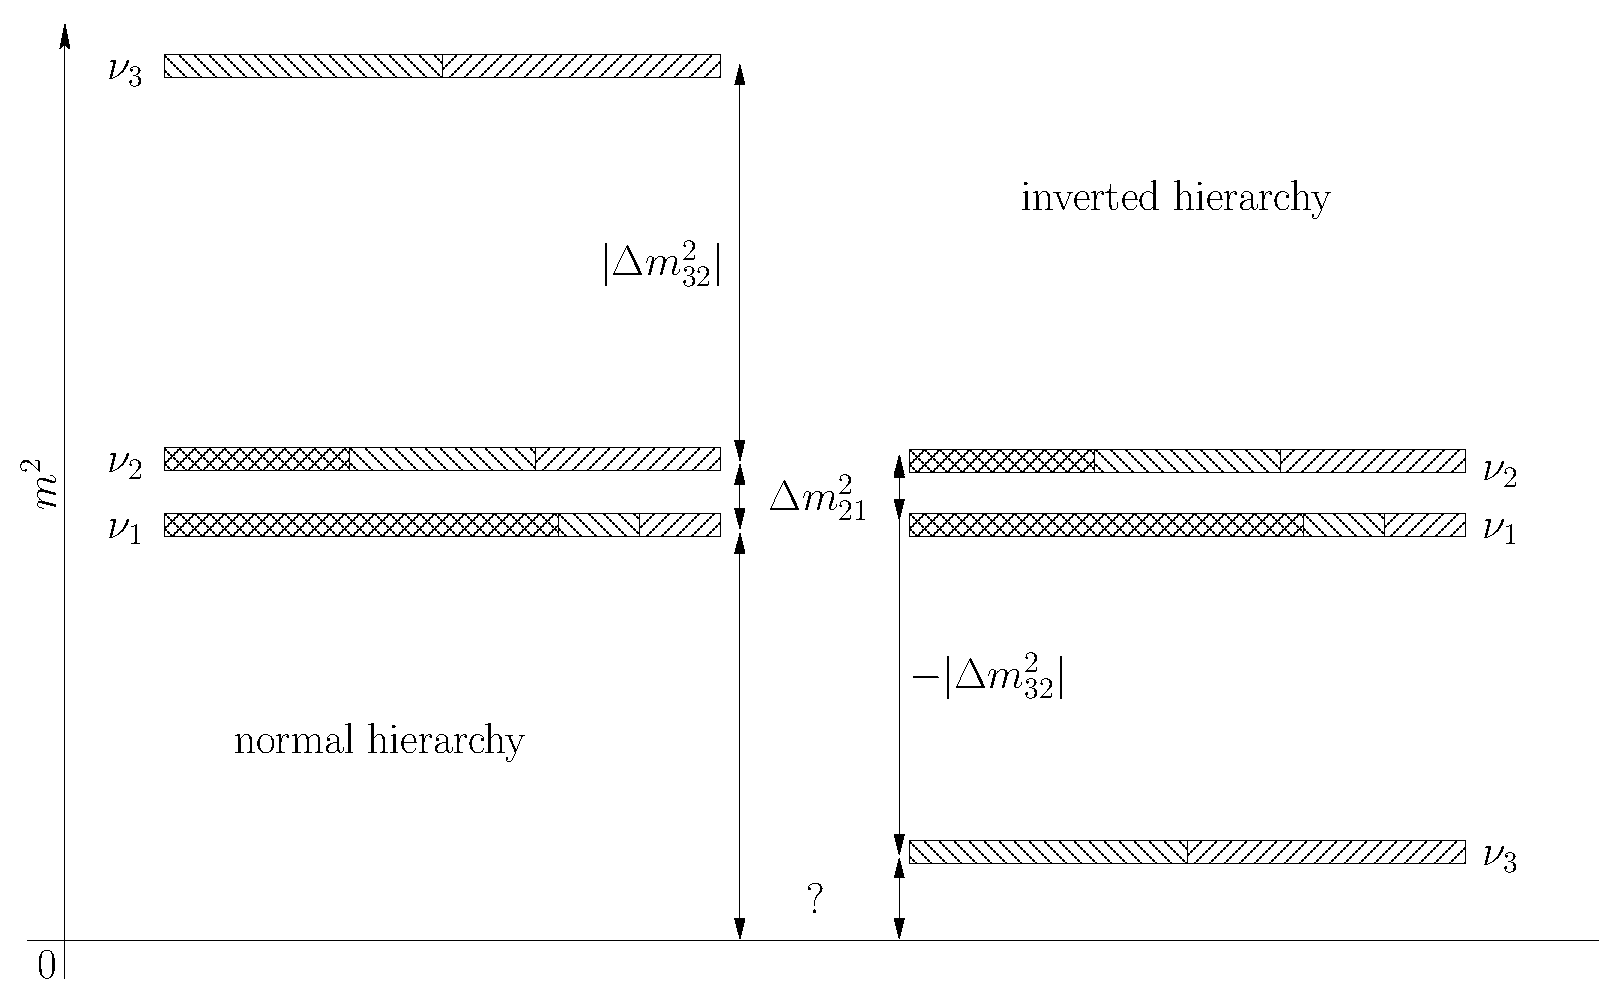
\includegraphics[width=0.8\textwidth]{massHierarchy.eps}  
  \caption{Possible neutrino squared-mass spectra. Oscillation    
experiments can neither tell how far above zero the entire spectra    
lie, nor the real mass hierarchy.}
  \label{fig:hie}
\end{figure}

\begin{table}[tbhp]
  \centering
  \caption{Summary of the neutrino squared-mass differences and the         
    mixing parameters based on the 3-neutrino mixing scheme. The         suffixes $_\odot$ and $_{\mbox{atm}}$ stand for the results from         solar and atmosphere experiments, respectively.}
  \label{tab:par}
  \begin{tabular}{lr}\hline\hline
    Parameter & Value \\\hline
    $\sin^{2}2\theta_{12} \approx \sin^{2}2\theta_{\odot}$ &    
$0.86^{+0.03}_{-0.04}$ \\
    $\sin^{2}2\theta_{23} \approx \sin^{2}2\theta_{\mbox{atm}}$ &        
$>0.92$ (C.L. = 90\%) \\
    $\sin^{2}2\theta_{13}$ & $<0.19$ (C.L. = 90\%) \\
    $\Delta m^{2}_{21}~[10^{-5}\mbox{eV}^{2}]$ & $0.8 \pm 0.3$ \\
    $|\Delta m^{2}_{32}|~[10^{-3}\mbox{eV}^{2}]$ & 1.9 to 3.0        
\\\hline\hline
  \end{tabular}
\end{table}

\section{Neutrino Mass Terms}
\label{sec:nema}
\subsection{Dirac neutrinos}
\label{sec:dirac}
The observation of neutrino oscillations makes the introduction of
neutrino mass terms into the \emph{Standard Model} necessary. In case
of free fields of fermions, the Dirac equation can be deduced from the
Lagrangian density
\begin{equation}
  \label{eq:deq}
  \mathcal{L} = \bar{\psi} (i\gamma^{\mu}\partial_{\mu}-m) \psi,
\end{equation}
where $\psi$ is the free Dirac field. The first term corresponds to
the kinetic energy and the second is the Dirac mass term,
\begin{equation}
  \label{eq:dm}
  \mathcal{L}_D=m_{D}\bar{\psi}\psi.
\end{equation}
Since
\begin{equation}
  \label{eq:2psi}
  \bar{\psi}\psi =  \bar{\psi}    
\left(\frac{1+\gamma^5}{2}+\frac{1-\gamma^5}{2}\right)
  \left(\frac{1+\gamma^5}{2}+\frac{1-\gamma^5}{2}\right) \psi =
  \bar{\psi}_{L}\psi_{R}+\bar{\psi}_{R}\psi_{L},
\end{equation}
a right-handed partner of the left-handed neutrino must be introduced
in order to prevent the above term vanishing. This particle does not
participate the weak interaction hence is called as the sterile
neutrino.

To motivate the above mass term, the most straightforward approach is
to follow the same procedure as for the electron, \textit{i.e.} the
lepton obtains mass by coupling to the Higgs field. The mass term of
the electron can be expressed as
\begin{equation}
  \label{eq:dme}
  m_{e}\bar{\psi_e}\psi_{e} = g_{e}\langle      
h^{0}\rangle\bar{\psi_e}\psi_{e},
\end{equation}
where $g_e$ is the coupling strength of electron field with Higgs
field, $\langle h^{0}\rangle$ is the vacuum expectation value for the
Higgs field. Similarly,
\begin{equation}
  \label{eq:dmnu}
  m_{\nu}\bar{\psi_\nu}\psi_{\nu} = g_{\nu}\langle  
h^{0}\rangle\bar{\psi_\nu}\psi_{\nu},
\end{equation}
where $g_\nu$ is the coupling strength of neutrino field with Higgs
field. Since neutrinos are much lighter than their leptonic partners,
the coupling strength of neutrino field with Higgs field should be
much smaller than that of electron:
\begin{equation}
  \label{eq:gg}
  g_{\nu} \ll g_{e}.
\end{equation}
By only introducing the Dirac mass term one has to answer the question
why neutrinos couple to the Higgs field so weakly compared with their
leptonic partners.

\subsection{Majorana neutrinos}
\label{sec:major}
Theoretically speaking, $\bar{\psi}^{c}\psi^{c}, \bar{\psi}\psi^{c}$
and $\bar{\psi}^{c}\psi$ are also possible mass terms, where
$\psi^{c}$ are the charge conjugate of $\psi$.
$\bar{\psi}^{c}\psi^{c}$ is equivalent to $\bar{\psi}\psi$.
$\bar{\psi}\psi^{c}$ and $\bar{\psi}^{c}\psi$ cannot be the mass terms
for electrons or quarks because it destroys or creates two particles
of the same charge. But nothing forbids to use them as mass terms for
neutrinos because neutrinos have no charge. These mass terms destroy
or creates two particles of the same lepton number hence violate
lepton number conservation, which is not necessarily to be true as
being discussed in section~\ref{sec:sm}.

After abandoning the lepton number conservation a generetic expression
of the mass term of one generation of neutrino is
\begin{equation}
  \label{eq:dmm}
  \mathcal{L}_{D+M} = m_{D}(\bar{\psi}_{L}\psi_{R} +  
\bar{\psi}^{c}_{L}\psi^{c}_{R}) +
  m_{L}\bar{\psi}_{L}\psi^{c}_{R} +   m_{R}\bar{\psi}^{c}_{L}\psi_{R}
+ h.c.,
\end{equation}
which can be reframed as
\begin{equation}
  \label{eq:mm}
  \mathcal{L}_{D+M} = (\bar{\psi}_{L},\bar{\psi}^{c}_{L})
  \left(\begin{array}{cc}m_L & m_D \\ m_D & m_R\end{array}\right)
  \left(\begin{array}{c}\psi^{c}_R \\ \psi_R\end{array}\right) + h.c.
\end{equation}
By choosing a orthogonal matrix $\mathcal{U}$ ($\mathcal{U}^{T}
\mathcal{U} = 1$) so that
\begin{equation}
  \label{eq:mmat}
  \mathcal{U}^{T}\left(\begin{array}{cc}m_L & m_D \\ m_D &       
m_R\end{array}\right)\mathcal{U} = 
  \left(\begin{array}{cc}\epsilon_{1}m_1 & 0 \\ 0 &            
\epsilon_{2}m_2\end{array}\right),
\end{equation}
where $m_{1}, m_{2} > 0$, $\epsilon_{1,2}$ indicate the signs of
$m_{1}, m_{2}$ and hence equal to $\pm 1$, and defining
\begin{equation}
  \label{eq:mvet}
  (\psi_{1L}, \psi_{2L}) = 
  (\bar{\psi}_{L}, \bar{\psi}^{c}_{L})~ \mathcal{U},
  \left(\begin{array}{c} \psi^{c}_{1R} \\            
\psi^{c}_{2R}\end{array}\right) = \mathcal{U}^{T}
  \left(\begin{array}{c} \psi^{c}_{R} \\ \psi_{R} \end{array}\right),
\end{equation}
eq.~\ref{eq:mm} can be rewritten as
\begin{equation}
  \label{eq:m12}
  \mathcal{L}_{D+M} = m_{1}\bar{\psi}_{1L}\psi^{c}_{1R} +  
m_{1}\bar{\psi}^{c}_{1R}\psi_{1L} +
  m_{2}\bar{\psi}_{2L}\psi^{c}_{2R} +  
m_{2}\bar{\psi}^{c}_{2R}\psi_{2L}.
\end{equation}
Define
\begin{equation}
  \label{eq:mafi}
  \phi_{1} = \psi_{1L} + \epsilon_{1}\psi^{c}_{1R}, 
  \mbox{\ \ \ and \ \ \ }
  \phi_{2} = \psi_{2L} + \epsilon_{2}\psi^{c}_{2R}.
\end{equation}
Eq.~\ref{eq:mm} can be rewritten as
\begin{equation}
  \label{eq:mv}
  \mathcal{L}_{D+M} = m_{1}\bar{\phi}_{1}\phi_{1} +
m_{2}\bar{\phi}_{2}\phi_{2}
\end{equation}
It is easy to find out that
\begin{equation}
  \label{eq:mach}
  \phi^{c}_{k} = (\psi_{kL})^{c} + \epsilon_{k}(\psi^{c}_{kR})^{c} =
\epsilon_{k}\phi_{k}, ~~~ (k=1,2)
\end{equation}
\textit{i.e.} $\psi$ is its own anti-particle, and hence of Majorana
type.

In case that $m_{R}$ is very heavy, $m_{L} = 0$ and $m_{D} \approx
\mathcal{O}(m_{e})$, we have
\begin{equation}
  \label{eq:seesaw}
  m_{1} = \frac{m^{2}_{D}}{m_{R}}\ll m_{D},  \mbox{\ \ \ and \ \ \ }  
m_{2} = m_{R}(1+\frac{m^{2}_{D}}{m^{2}_{R}}) \approx m_{R} \gg m_{D}.
\end{equation}
\textit{i.e.} if there exists a very heavy Majorana neutrino $\phi_2$,
the other Majorana neutrino would be much lighter than $m_e$. This is
so-called seesaw machenism.

To sum up, Majorana mass terms should be taken into account in general
as well as Dirac mass terms. For fermions carrying charge or similar
quantum numbers the former mass terms are forbidden, while this is not
the case for neutrinos. Majorana neutrinos $\phi_{1}, \phi_{2}$ can be
constructed out of Dirac fields. By using seesaw mechanism the tiny
neutrino mass can be explained naturally.

\section{Double beta decay}
\label{sec:0n2b}
If neutrinos are of Majorana type the two neutrinos from double beta
decay ($2\nu\beta\beta$) as shown in eq.~\ref{eq:2nu2b} may annihilate
with each other. This is the so-called neutrinoless double beta decay
($0\nu\beta\beta$) as shown in eq.~\ref{eq:0nu2b}:
\begin{eqnarray}
  2\nu\beta\beta: &(Z,A)& \rightarrow (Z+2,A) + 2e^{-} +
2\bar{\nu}_{e}, \\\label{eq:2nu2b}
  0\nu\beta\beta: &(Z,A)& \rightarrow (Z+2,A) + 2e^{-},
\label{eq:0nu2b}
\end{eqnarray}
where $Z$ is the charge of the nucleus and $A$ is the atomic number.
The Feynman diagrams of both processes are shown in
Fig.~\ref{fig:2bdecay}.
\begin{figure}[tbhp]
  \centering
  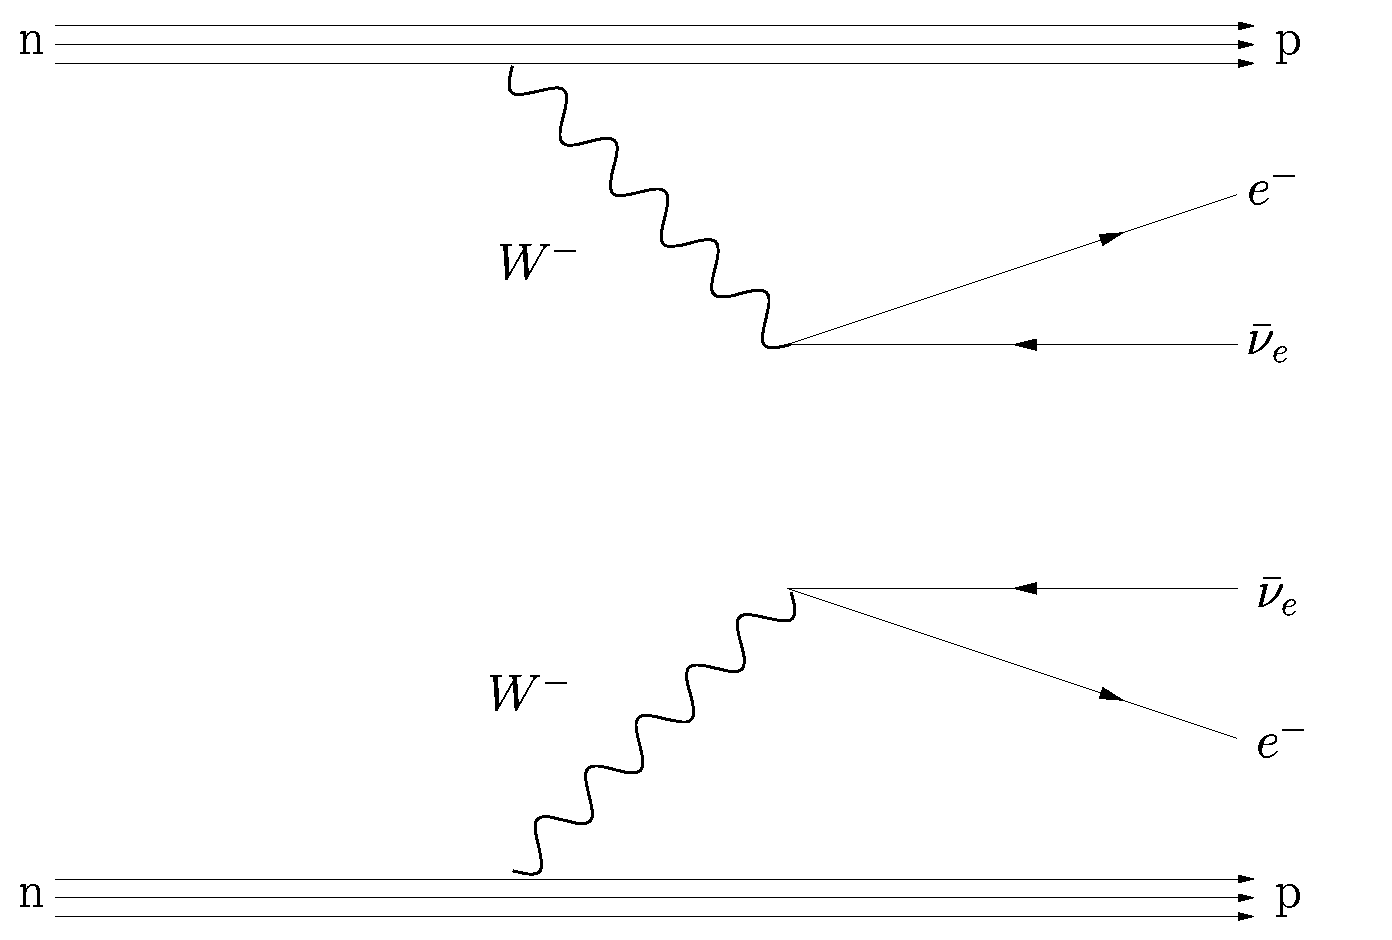
\includegraphics[width=0.45\textwidth]{FD2nu2b.eps} \hfil
  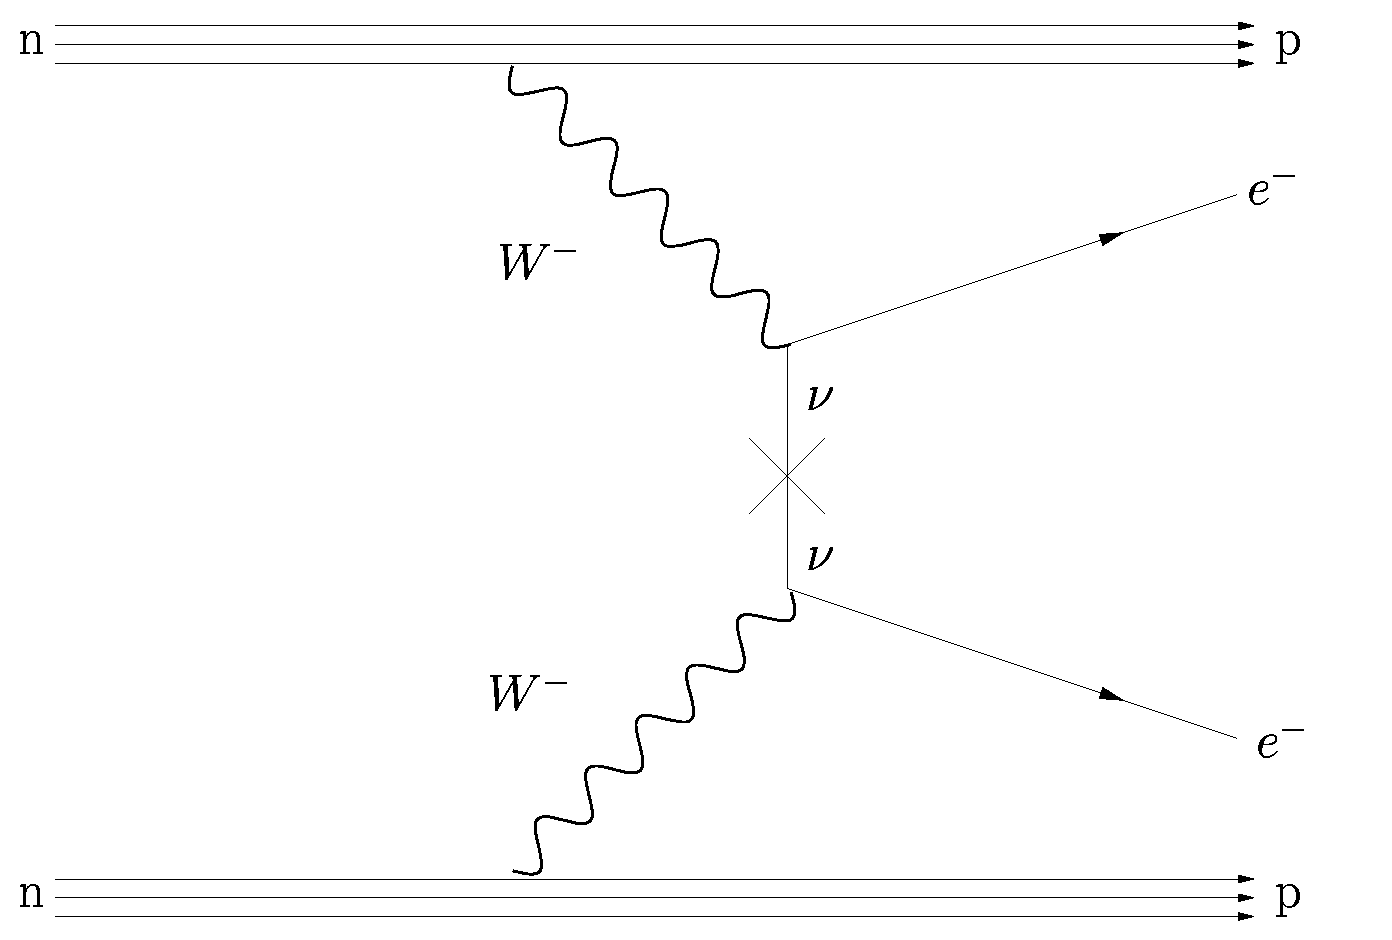
\includegraphics[width=0.45\textwidth]{FD0nu2b.eps}  
  \caption{Feynman diagrams of double beta decay with and without two neutrinos being emitted.}
  \label{fig:2bdecay}
\end{figure}

\subsection{Double beta decay with neutrinos}
\label{sec:2n2b}
The study of double beta decay started in 1935~\cite{Goe35} when Maria
Goeppert-Mayer applied Fermi's beta decay theory to calculate the
process as shown in eq.~\ref{eq:2nu2b} as a second order effect. According to Fermi's golden rule the rate of double beta decay is 
\begin{equation}
  \label{eq:2nurate}
  1/T^{2\nu}_{1/2} = G_{2\nu}(Q,Z) |\mathcal{M}_{2\nu}|^{2},
\end{equation}
where the phase space factor $G_{2\nu}(Q,Z)$ depends on the $Q$-value and the nuclear charge $Z$, the nuclear matrix element $\mathcal{M}_{2\nu}$ describes the hadronic part of the decay. Maria's motivation had nothing to do with neutrinos. She was concerned with the stability of various even-even nuclei over geological time. These nuclei, consisting of even numbers of protons and neutrons, cannot decay into their nearest neighbor even-odd nuclei due to energy conservation. They can however decay into their next nearest neighbors, as shown in Fig.~\ref{fig:ee2oo}. More than 60 naturally occurring isotopes should be able to undergo double-beta decay. Only ten of them were observed to actually do it. They are $^{48}$Ca, $^{76}$Ge, $^{82}$Se, $^{96}$Zr, $^{100}$Mo, $^{116}$Cd, $^{128}$Te, $^{130}$Te, $^{150}$Nd, and $^{238}$U. A comprehensive list of the decay modes and the corresponding lifetime of each isotope can be found in the latest \emph{Review of Particle Physics}~\cite{PDG07}.
\begin{figure}[tbhp]
  \centering
  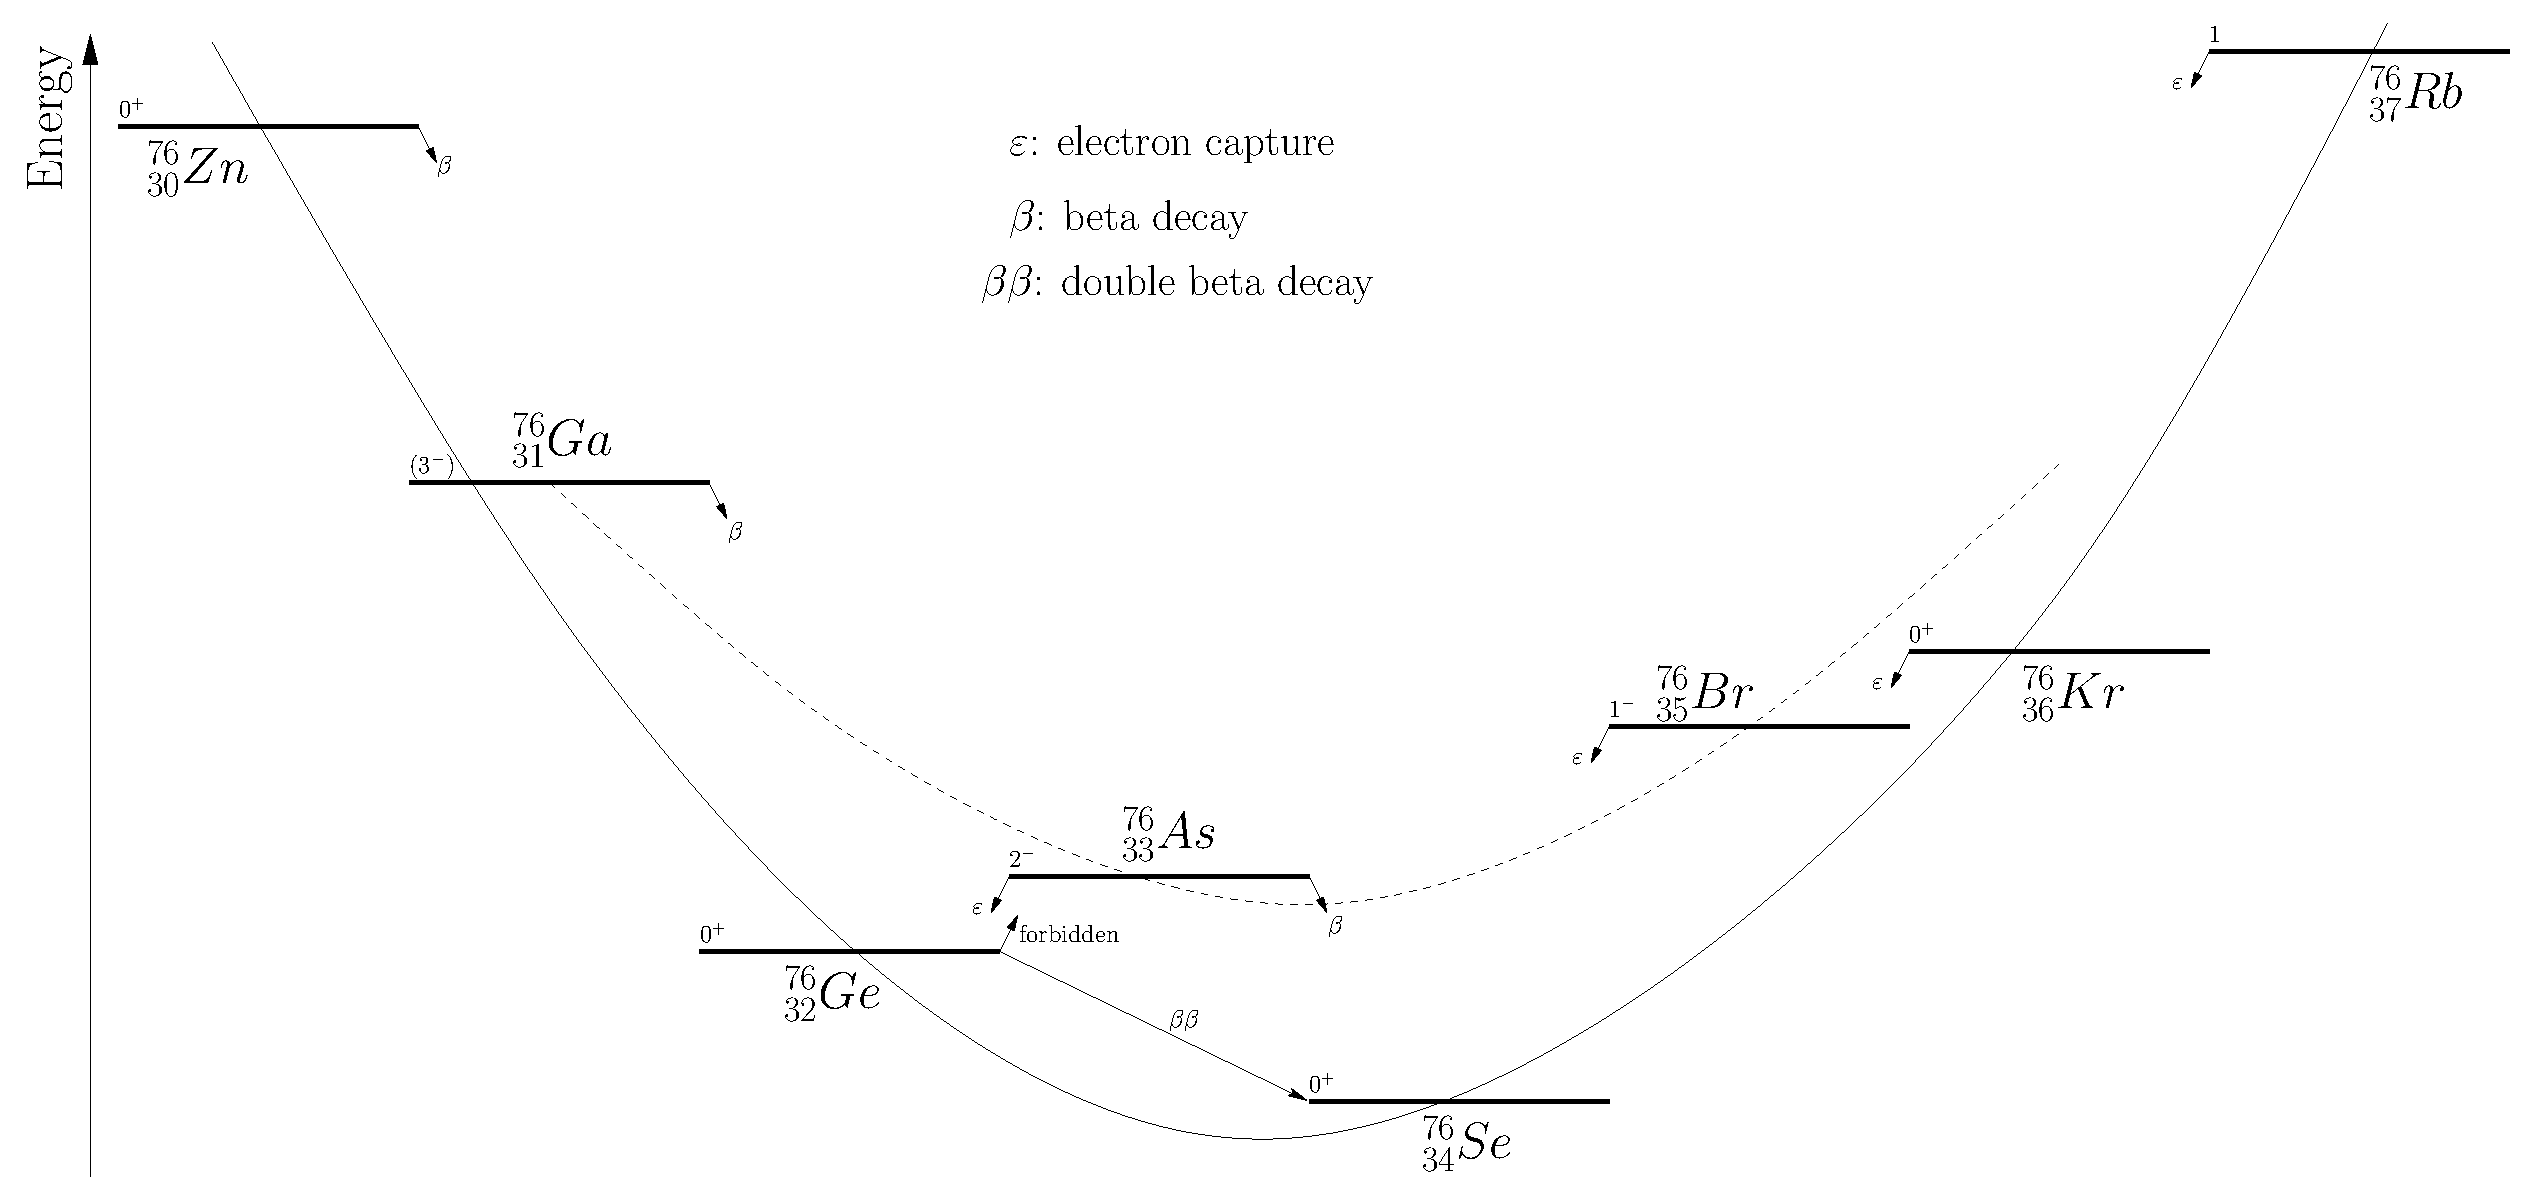
\includegraphics[width=0.6\textwidth]{Espec0nu2b.eps}  
  \caption{Energy scheme for the double beta decay from parent nucleus     $^{A}X$ to daughter nucleus $^{A}Y$. The single beta decay to the     intermediate isotope $^{A}T$ is forbidden due to the energy     conservation.}
  \label{fig:ee2oo}
\end{figure}

\subsection{Neutrinoless double beta decay}
\label{sec:0n2brate}
The study of neutrinoless double beta decay started several years
later~\cite{Rac37,Fur37} when W. H. Furry showed that Majorana's
symmetrical theory of neutrino and anti-neutrino could give rise to a
neutrinoless mode of double beta decay. Prior to the discovery of
parity non-conservation, the lifetime of neutrinoless double beta
decay was calculated incorrectly. The understanding of double beta
decay changed profoundly when parity non-conservation was discovered
in 1957 and the two-component theory of the neutrino was developed.
According to the two-component theory the probability for neutrinoless
double beta decay via Furry's mechanism is zero because the neutrino
emitted in the first beta decay is in the wrong helicity state to
stimulate a second beta decay process. The observation of neutrino
oscillations changed the picture once again. The rate of neutrinoless
double beta decay can be expressed as
\begin{equation}
  \label{eq:0nura}
  1/T^{0\nu}_{1/2} = \sum_{\text{spins}} \int |Z_{0\nu}|^{2}
\delta(E_{e1} + E_{e2} + Q_{\beta\beta})
\frac{d^{3}p_{e1}}{(2\pi)^{3}} \frac{d^{3}p_{e2}}{(2\pi)^{3}},
\end{equation}
where $Q_{\beta\beta}$ is the Q-value of the decay, $E_{e1}, E_{e2},
p_{e1}, p_{e2}$ are the energies and momenta of the outgoing electrons
and $Z_{0\nu}$ is the transition amplitude. $Z_{0\nu}$ contains both
leptonic and hadronic parts. Taking into account the neutrino mixing
the leptonic part is of the form
\begin{equation}
  \label{eq:leppar}
  \contraction{\sum_{k}\bar{e}(x)\gamma_{\mu}(1-\gamma_{5})U_{ek}}
  {\phi}{{}_{k}(x)\bar{e}(y)\gamma_{\nu}(1-\gamma_{5})U_{ek}}{\phi}
  \sum_{k}\bar{e}(x)\gamma_{\mu}(1-\gamma_{5})U_{ek}\phi_{k}(x)
  \bar{e}(y)\gamma_{\nu}(1-\gamma_{5})U_{ek}\phi_{k}(y).
\end{equation}
Assuming only the exchange of three light neutrinos, the leptonic part
is proportional to 
\begin{equation}
  \label{eq:effmass}
  \langle m_{\nu_{e}} \rangle \equiv \left| \sum_{k}m_{k}U^{2}_{ek}
\right| = \left| m_{1}|U_{e1}|^{2} +
m_{2}|U_{e2}|^{2}e^{i(\alpha_{2}-\alpha_{1})} +
m_{3}|U_{e3}|^{2}e^{-i(\alpha_{1}+2\delta)} \right|,
\end{equation}
where $\langle m_{\nu_{e}} \rangle$ is called the effective Majorana
neutrino mass. The rate of neutrinoless double beta decay can be
expressed in term of the effective Majorana neutrino mass as
\begin{equation}
  \label{eq:0nurate}
  1/T^{0\nu}_{1/2} = G_{0\nu}(Q,Z) |\mathcal{M}_{0\nu}|^{2} \langle
m_{\nu_{e}} \rangle^{2},
\end{equation}
where $G_{0\nu}(Q,Z)$ is the phase space factor, $\mathcal{M}_{0\nu}$
denotes the nuclear matrix elements which describe the hadronic part
of the decay. 

If the neutrino squared-mass spectrum is of the normal order, as shown
in the left plot of Fig.~\ref{fig:hie}, the effective Majorana
neutrino mass could be invisibly small. Because the terms in
eq.~\ref{eq:effmass} can cancel each other out if the CP-violation
phases $\alpha_{1}, \alpha_{2}$ and $\delta$ take some special values.
Fig.~\ref{fig:effmvmm} taken from Ref.~\cite{Mer06} shows the
effective Majorana neutrino mass as a function of the lightest
neutrino mass. The mixing angle $\theta_{13}$ is assumed to be zero.
The light band corresponds to the inverted mass hierarchy, the dark
band to the normal mass hierarchy. An experiment sensitive to $\langle
m_{\nu_{e}} \rangle \sim 10$meV has an excellent chance to seeing a
signal in case of inverted mass hierarchy. And if the observed
$\langle m_{\nu_{e}} \rangle$ is far below $10$meV the inverted mass
hierarchy can be ruled out.
\begin{figure}[tbhp]
  \centering
  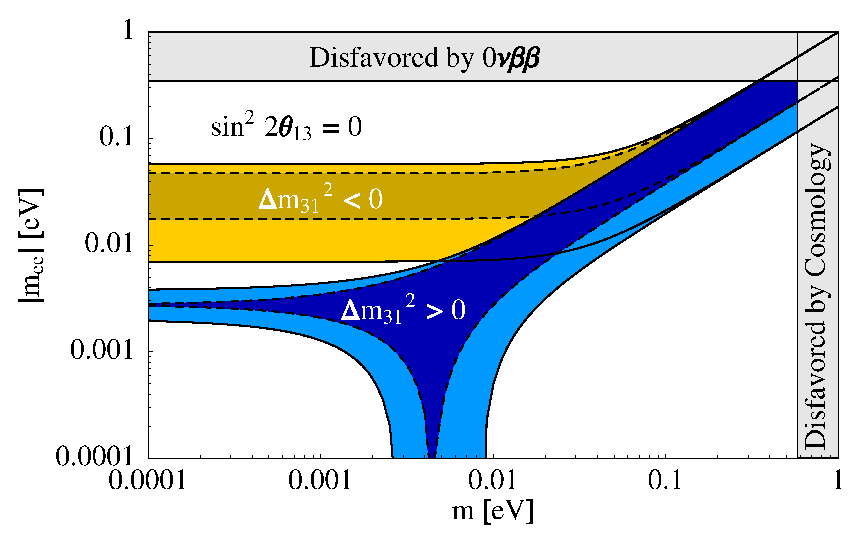
\includegraphics[width=0.8\textwidth]{mnueVm.eps}  
  \caption{The effective Majorana neutrino mass as a function of the
lightest neutrino mass, m. The mixing angle $\theta_{13}$ is assumed
to be zero. The light band corresponds to the inverted mass hierarchy,
the dark band to the normal mass hierarchy. the inner/outer bands
correspond to calculations without/with the $3\sigma$-uncertainties on
the oscillation parameters. }
  \label{fig:effmvmm}
\end{figure}

\subsection{Double beta decay experiments}
\label{sec:genremark}
Q-value, nuclear matrix, natural abundance, background, efficiency ...

comparison between different double beta decay experiments.

\subsection{Neutrinoless double beta decay of $^{76}$Ge}
\label{sec:ge76}

advantage of $^{76}$Ge.

IGEX and Heidelberg-Moscow.

\section{Other aspects of neutrino physics}
\label{sec:others}

\subsection{Seesaw mechanism}
\label{sec:seesaw}
the problems of seesaw mechanism

\subsection{Neutrino pair production}
\label{sec:pair}
the cross sections are different if neutrinos are of different type.

\subsection{Neutrino magnetic moment}
\label{sec:mag}
if neutrino has magnetic moment, it cannot be of Majorana type.

\subsection{Neutrinos in astrophysics}
\label{sec:astro}
mass and number of types of neutrinos



%%% Local Variables:
%%% mode:latex
%%% TeX-master: "thesis"
%%% End:
